% Options for packages loaded elsewhere
\PassOptionsToPackage{unicode}{hyperref}
\PassOptionsToPackage{hyphens}{url}
%
\documentclass[
  11pt]{report}
\usepackage{amsmath,amssymb}
\usepackage{lmodern}
\usepackage{iftex}
\ifPDFTeX
  \usepackage[T1]{fontenc}
  \usepackage[utf8]{inputenc}
  \usepackage{textcomp} % provide euro and other symbols
\else % if luatex or xetex
  \usepackage{unicode-math}
  \defaultfontfeatures{Scale=MatchLowercase}
  \defaultfontfeatures[\rmfamily]{Ligatures=TeX,Scale=1}
\fi
% Use upquote if available, for straight quotes in verbatim environments
\IfFileExists{upquote.sty}{\usepackage{upquote}}{}
\IfFileExists{microtype.sty}{% use microtype if available
  \usepackage[]{microtype}
  \UseMicrotypeSet[protrusion]{basicmath} % disable protrusion for tt fonts
}{}
\makeatletter
\@ifundefined{KOMAClassName}{% if non-KOMA class
  \IfFileExists{parskip.sty}{%
    \usepackage{parskip}
  }{% else
    \setlength{\parindent}{0pt}
    \setlength{\parskip}{6pt plus 2pt minus 1pt}}
}{% if KOMA class
  \KOMAoptions{parskip=half}}
\makeatother
\usepackage{xcolor}
\IfFileExists{xurl.sty}{\usepackage{xurl}}{} % add URL line breaks if available
\IfFileExists{bookmark.sty}{\usepackage{bookmark}}{\usepackage{hyperref}}
\hypersetup{
  pdftitle={Introduction to Probability (Joe Blitzstein)},
  pdfauthor={Fernando Náufel},
  pdflang={pt-br},
  hidelinks,
  pdfcreator={LaTeX via pandoc}}
\urlstyle{same} % disable monospaced font for URLs
\usepackage[margin=1in]{geometry}
\usepackage{color}
\usepackage{fancyvrb}
\newcommand{\VerbBar}{|}
\newcommand{\VERB}{\Verb[commandchars=\\\{\}]}
\DefineVerbatimEnvironment{Highlighting}{Verbatim}{commandchars=\\\{\}}
% Add ',fontsize=\small' for more characters per line
\usepackage{framed}
\definecolor{shadecolor}{RGB}{248,248,248}
\newenvironment{Shaded}{\begin{snugshade}}{\end{snugshade}}
\newcommand{\AlertTok}[1]{\textcolor[rgb]{0.94,0.16,0.16}{#1}}
\newcommand{\AnnotationTok}[1]{\textcolor[rgb]{0.56,0.35,0.01}{\textbf{\textit{#1}}}}
\newcommand{\AttributeTok}[1]{\textcolor[rgb]{0.77,0.63,0.00}{#1}}
\newcommand{\BaseNTok}[1]{\textcolor[rgb]{0.00,0.00,0.81}{#1}}
\newcommand{\BuiltInTok}[1]{#1}
\newcommand{\CharTok}[1]{\textcolor[rgb]{0.31,0.60,0.02}{#1}}
\newcommand{\CommentTok}[1]{\textcolor[rgb]{0.56,0.35,0.01}{\textit{#1}}}
\newcommand{\CommentVarTok}[1]{\textcolor[rgb]{0.56,0.35,0.01}{\textbf{\textit{#1}}}}
\newcommand{\ConstantTok}[1]{\textcolor[rgb]{0.00,0.00,0.00}{#1}}
\newcommand{\ControlFlowTok}[1]{\textcolor[rgb]{0.13,0.29,0.53}{\textbf{#1}}}
\newcommand{\DataTypeTok}[1]{\textcolor[rgb]{0.13,0.29,0.53}{#1}}
\newcommand{\DecValTok}[1]{\textcolor[rgb]{0.00,0.00,0.81}{#1}}
\newcommand{\DocumentationTok}[1]{\textcolor[rgb]{0.56,0.35,0.01}{\textbf{\textit{#1}}}}
\newcommand{\ErrorTok}[1]{\textcolor[rgb]{0.64,0.00,0.00}{\textbf{#1}}}
\newcommand{\ExtensionTok}[1]{#1}
\newcommand{\FloatTok}[1]{\textcolor[rgb]{0.00,0.00,0.81}{#1}}
\newcommand{\FunctionTok}[1]{\textcolor[rgb]{0.00,0.00,0.00}{#1}}
\newcommand{\ImportTok}[1]{#1}
\newcommand{\InformationTok}[1]{\textcolor[rgb]{0.56,0.35,0.01}{\textbf{\textit{#1}}}}
\newcommand{\KeywordTok}[1]{\textcolor[rgb]{0.13,0.29,0.53}{\textbf{#1}}}
\newcommand{\NormalTok}[1]{#1}
\newcommand{\OperatorTok}[1]{\textcolor[rgb]{0.81,0.36,0.00}{\textbf{#1}}}
\newcommand{\OtherTok}[1]{\textcolor[rgb]{0.56,0.35,0.01}{#1}}
\newcommand{\PreprocessorTok}[1]{\textcolor[rgb]{0.56,0.35,0.01}{\textit{#1}}}
\newcommand{\RegionMarkerTok}[1]{#1}
\newcommand{\SpecialCharTok}[1]{\textcolor[rgb]{0.00,0.00,0.00}{#1}}
\newcommand{\SpecialStringTok}[1]{\textcolor[rgb]{0.31,0.60,0.02}{#1}}
\newcommand{\StringTok}[1]{\textcolor[rgb]{0.31,0.60,0.02}{#1}}
\newcommand{\VariableTok}[1]{\textcolor[rgb]{0.00,0.00,0.00}{#1}}
\newcommand{\VerbatimStringTok}[1]{\textcolor[rgb]{0.31,0.60,0.02}{#1}}
\newcommand{\WarningTok}[1]{\textcolor[rgb]{0.56,0.35,0.01}{\textbf{\textit{#1}}}}
\usepackage{longtable,booktabs,array}
\usepackage{calc} % for calculating minipage widths
% Correct order of tables after \paragraph or \subparagraph
\usepackage{etoolbox}
\makeatletter
\patchcmd\longtable{\par}{\if@noskipsec\mbox{}\fi\par}{}{}
\makeatother
% Allow footnotes in longtable head/foot
\IfFileExists{footnotehyper.sty}{\usepackage{footnotehyper}}{\usepackage{footnote}}
\makesavenoteenv{longtable}
\setlength{\emergencystretch}{3em} % prevent overfull lines
\providecommand{\tightlist}{%
  \setlength{\itemsep}{0pt}\setlength{\parskip}{0pt}}
\setcounter{secnumdepth}{5}
\newlength{\cslhangindent}
\setlength{\cslhangindent}{1.5em}
\newlength{\csllabelwidth}
\setlength{\csllabelwidth}{3em}
\newlength{\cslentryspacingunit} % times entry-spacing
\setlength{\cslentryspacingunit}{\parskip}
\newenvironment{CSLReferences}[2] % #1 hanging-ident, #2 entry spacing
 {% don't indent paragraphs
  \setlength{\parindent}{0pt}
  % turn on hanging indent if param 1 is 1
  \ifodd #1
  \let\oldpar\par
  \def\par{\hangindent=\cslhangindent\oldpar}
  \fi
  % set entry spacing
  \setlength{\parskip}{#2\cslentryspacingunit}
 }%
 {}
\usepackage{calc}
\newcommand{\CSLBlock}[1]{#1\hfill\break}
\newcommand{\CSLLeftMargin}[1]{\parbox[t]{\csllabelwidth}{#1}}
\newcommand{\CSLRightInline}[1]{\parbox[t]{\linewidth - \csllabelwidth}{#1}\break}
\newcommand{\CSLIndent}[1]{\hspace{\cslhangindent}#1}
\ifLuaTeX
\usepackage[bidi=basic]{babel}
\else
\usepackage[bidi=default]{babel}
\fi
\babelprovide[main,import]{brazilian}
% get rid of language-specific shorthands (see #6817):
\let\LanguageShortHands\languageshorthands
\def\languageshorthands#1{}

% A command to save the path to the resources of bd.format (fnaufel)
\newcommand{\dir}{/ssd/R/x86_64-pc-linux-gnu-library/4.1/fnaufelRmd/rmarkdown/resources}



\hypersetup{
  colorlinks,
  breaklinks,
  linkcolor=magenta,
  urlcolor=blue
}

% Lexend font
\usepackage{lexend}


% Para bibliografia em português
\usepackage{babelbib}

% Para títulos de capítulos e seções:
\usepackage[nobottomtitles*]{titlesec}

%%%%%%%%%%%%%%%
%
% Titulos de capítulos e seções

\titleformat{\chapter}[display]%
{\bfseries\Large}%
{\filleft\MakeUppercase{\chaptertitlename} \Huge\thechapter}%
{4ex}%
{\titlerule%
  \vspace{2ex}%
  \filright}%
[\vspace{2ex}%
\titlerule%
\vspace{10ex}]

\titleformat{\section}[block]%
{\bfseries\Large}%
{\thesection}{.5em}{\titlerule\\[.8ex]\bfseries}

\titleformat{\subsection}[block]%
{\bfseries}%
{\thesubsection}{.5em}{\titlerule\\[.8ex]\bfseries}%
[\vspace{1ex}]

%%%%%%%%%%%%%%%
%
% Caixas

\usepackage{tcolorbox}

\tcbset{
  rounded corners,
  boxrule=0.3mm,
  colback=black!.5!white,
  parbox=false
}

\newtcolorbox{rmdbox}{
  colframe=black!40!white,
}


\newtcolorbox{mycaution}{
  colframe=red!75!black,
  sidebyside,
  lower separated=false,
  lefthand width=1cm,
  sidebyside gap=4mm
}

\newenvironment{rmdcaution}
{
  \begin{mycaution}
    
\includegraphics[width=.8cm]{\dir/images/caution.png}
    \tcblower
  }
  {
  \end{mycaution}
}

\newtcolorbox{myimportant}{
  colframe=green!75!black,
  sidebyside,
  lower separated=false,
  lefthand width=1cm,
  sidebyside gap=4mm
}

\newenvironment{rmdimportant}
{
  \begin{myimportant}
    
\includegraphics[width=.8cm]{\dir/images/important.png}
    \tcblower
  }
  {
  \end{myimportant}
}

\newtcolorbox{mywarning}{
  colframe=yellow!80!black,
  sidebyside,
  lower separated=false,
  lefthand width=1cm,
  sidebyside gap=4mm
}

\newenvironment{rmdwarning}
{
  \begin{mywarning}
    
\includegraphics[width=.8cm]{\dir/images/warning.png}
    \tcblower
  }
  {
  \end{mywarning}
}

\newtcolorbox{mynote}{
  colframe=yellow!70!black,
  sidebyside,
  lower separated=false,
  lefthand width=1cm,
  sidebyside gap=4mm
}

\newenvironment{rmdnote}
{
  \begin{mynote}
    
\includegraphics[width=.8cm]{\dir/images/note.png}
    \tcblower
  }
  {
  \end{mynote}
}

\newtcolorbox{mytip}{
  colframe=blue!50!white,
  sidebyside,
  lower separated=false,
  lefthand width=1cm,
  sidebyside gap=4mm
}

\newenvironment{rmdtip}
{
  \begin{mytip}
    
\includegraphics[width=.8cm]{\dir/images/tip.png}
    \tcblower
  }
  {
  \end{mytip}
}

% For highlighting using \hl{}
\usepackage{soul}


\makeatletter
\@ifundefined{Shaded}{}{
  % Code chunks and output
  \usepackage[framemethod=pgf]{mdframed}
  \renewenvironment{Shaded}{
    \begin{mdframed}[%
      roundcorner=2pt,%
      innerleftmargin=5pt,%
      innerrightmargin=5pt,%
      topline=true,%
      leftline=true,%
      rightline=true,%
      bottomline=true,%
      linewidth=0.5pt,%
      linecolor=black!20,%
      backgroundcolor=black!2,%
      skipabove=2ex,%
      skipbelow=2.5ex%
    ]%
  }
  {
    \end{mdframed}
  }
}
\makeatother

% End of preamble for bookdowntemplate01

%%%%%%%%%%%%%%%%%%%%%%%%%%%%%%%%%%%%%%%%%%%%%%%%%%%%%%

\usepackage{booktabs}
\usepackage{longtable}
\usepackage{array}
\usepackage{multirow}
\usepackage{wrapfig}
\usepackage{float}
\usepackage{colortbl}
\usepackage{pdflscape}
\usepackage{tabu}
\usepackage{threeparttable}
\usepackage{threeparttablex}
\usepackage[normalem]{ulem}
\usepackage{makecell}
\usepackage{xcolor}
\ifLuaTeX
  \usepackage{selnolig}  % disable illegal ligatures
\fi

\title{Introduction to Probability (Joe Blitzstein)}
\author{Fernando Náufel}
\date{(versão de 07/02/2022)}

\begin{document}
\maketitle

{
\setcounter{tocdepth}{1}
\tableofcontents
}
\hypertarget{apresentauxe7uxe3o}{%
\chapter*{Apresentação}\label{apresentauxe7uxe3o}}
\addcontentsline{toc}{chapter}{Apresentação}

\begin{itemize}
\item
  Página do livro: \url{https://projects.iq.harvard.edu/stat110/home}
\item
  Strategic practice and homework: \url{https://projects.iq.harvard.edu/stat110/strategic-practice-problems}
\item
  Handouts: \url{https://projects.iq.harvard.edu/stat110/handouts} --- includes solutions to exercises marked with (s) in the book.
\item
  Playlist: \url{https://www.youtube.com/playlist?list=PL2SOU6wwxB0uwwH80KTQ6ht66KWxbzTIo}
\end{itemize}

\hypertarget{probabilidade-e-contagem}{%
\chapter*{01: Probabilidade e contagem}\label{probabilidade-e-contagem}}
\addcontentsline{toc}{chapter}{01: Probabilidade e contagem}

\hypertarget{vuxeddeo}{%
\section*{Vídeo}\label{vuxeddeo}}
\addcontentsline{toc}{section}{Vídeo}

\begin{center} \url{https://youtu.be/KbB0FjPg0mw} \end{center}

\hypertarget{pascal-e-fermat}{%
\section*{Pascal e Fermat}\label{pascal-e-fermat}}
\addcontentsline{toc}{section}{Pascal e Fermat}

\begin{itemize}
\item
  Ver artigo DEVLIN (\protect\hyperlink{ref-devlin-2010-pascal-fermat}{2010}).
\item
  Ver \href{https://gallica.bnf.fr/ark:/12148/bpt6k69975r.image.r=Blaise+Pascal.f233.langFR}{originais em francês de toda a correspondência de Pascal}.
\end{itemize}

\hypertarget{r}{%
\section*{R}\label{r}}
\addcontentsline{toc}{section}{R}

\hypertarget{fatoriais-e-combinauxe7uxf5es}{%
\subsection*{Fatoriais e combinações}\label{fatoriais-e-combinauxe7uxf5es}}
\addcontentsline{toc}{subsection}{Fatoriais e combinações}

\begin{itemize}
\item
  Qual o maior valor de $n$ para o qual o R calcula \texttt{factorial(n)}?

  No meu computador, $n = 170$:

\begin{Shaded}
\begin{Highlighting}[]
\FunctionTok{factorial}\NormalTok{(}\DecValTok{170}\SpecialCharTok{:}\DecValTok{171}\NormalTok{)}
\DocumentationTok{\#\# [1] 7,257416e+306           Inf}
\end{Highlighting}
\end{Shaded}
\item
  Para valores maiores, podemos usar \texttt{lfactorial(n)} para calcular $\ln n!$:

\begin{Shaded}
\begin{Highlighting}[]
\FunctionTok{lfactorial}\NormalTok{(}\DecValTok{170}\SpecialCharTok{:}\DecValTok{171}\NormalTok{)}
\DocumentationTok{\#\# [1] 706,5731 711,7147}
\end{Highlighting}
\end{Shaded}
\item
  Da mesma forma, \texttt{lchoose(n,\ k)} calcula $\ln \binom nk$.
\end{itemize}

\hypertarget{tabulando-dados-tabulate-times-table}{%
\subsection*{\texorpdfstring{Tabulando dados: \texttt{tabulate} $\times$ \texttt{table}}{Tabulando dados: tabulate  table}}\label{tabulando-dados-tabulate-times-table}}
\addcontentsline{toc}{subsection}{Tabulando dados: \texttt{tabulate} $\times$ \texttt{table}}

\begin{Shaded}
\begin{Highlighting}[]
\NormalTok{b }\OtherTok{\textless{}{-}} \FunctionTok{sample}\NormalTok{(}\DecValTok{1}\SpecialCharTok{:}\DecValTok{365}\NormalTok{,}\DecValTok{23}\NormalTok{,}\AttributeTok{replace=}\ConstantTok{TRUE}\NormalTok{)}
\FunctionTok{tabulate}\NormalTok{(b)}
\DocumentationTok{\#\#   [1] 0 0 0 0 0 0 0 0 0 0 0 0 0 0 0 0 0 0 0 0 0 0 0 0 0 0 0 0 0 0 0 0 0}
\DocumentationTok{\#\#  [34] 0 1 0 0 0 0 0 0 0 0 0 0 0 0 0 0 0 0 0 0 0 0 0 0 0 0 0 0 0 0 0 0 0}
\DocumentationTok{\#\#  [67] 0 0 0 0 0 0 0 0 0 0 0 0 1 0 0 0 1 0 1 0 0 0 0 0 0 0 0 0 0 0 0 0 0}
\DocumentationTok{\#\# [100] 0 0 0 0 0 0 0 0 0 0 0 0 0 0 0 0 0 0 0 0 0 1 0 0 0 0 0 0 1 0 0 0 0}
\DocumentationTok{\#\# [133] 0 0 0 0 0 0 0 0 0 0 0 0 0 0 0 1 0 0 0 0 0 0 0 0 0 1 0 0 1 0 0 0 0}
\DocumentationTok{\#\# [166] 0 0 0 0 0 1 0 0 0 0 1 0 0 0 0 0 0 0 0 0 0 1 0 0 0 0 0 0 0 0 0 0 0}
\DocumentationTok{\#\# [199] 0 0 0 0 0 0 0 0 0 0 0 0 0 0 0 0 0 0 0 0 0 0 1 0 0 0 0 0 0 0 0 0 0}
\DocumentationTok{\#\# [232] 0 0 0 0 0 0 0 1 0 1 0 0 0 0 0 0 0 0 0 1 0 0 1 0 0 0 0 0 1 0 0 0 0}
\DocumentationTok{\#\# [265] 0 0 0 0 0 0 1 0 0 0 0 0 0 0 0 0 0 0 0 0 0 0 0 0 0 0 0 0 0 0 0 0 0}
\DocumentationTok{\#\# [298] 0 0 0 0 0 0 0 0 0 0 0 0 0 0 0 0 0 0 0 0 0 0 0 0 0 0 0 0 0 0 0 1 0}
\DocumentationTok{\#\# [331] 0 0 0 0 0 0 0 0 0 1 1 0 0 0 0 0 0 0 0 0 0 0 1}
\end{Highlighting}
\end{Shaded}

\begin{Shaded}
\begin{Highlighting}[]
\FunctionTok{table}\NormalTok{(b)}
\DocumentationTok{\#\# b}
\DocumentationTok{\#\#  35  79  83  85 121 128 148 158 161 171 176 187 221 239 241 251 254 }
\DocumentationTok{\#\#   1   1   1   1   1   1   1   1   1   1   1   1   1   1   1   1   1 }
\DocumentationTok{\#\# 260 271 329 340 341 353 }
\DocumentationTok{\#\#   1   1   1   1   1   1}
\end{Highlighting}
\end{Shaded}

\hypertarget{funuxe7uxf5es-para-o-problema-do-aniversuxe1rio}{%
\subsection*{Funções para o problema do aniversário}\label{funuxe7uxf5es-para-o-problema-do-aniversuxe1rio}}
\addcontentsline{toc}{subsection}{Funções para o problema do aniversário}

\begin{Shaded}
\begin{Highlighting}[]
\FunctionTok{pbirthday}\NormalTok{(}\DecValTok{23}\NormalTok{)}
\DocumentationTok{\#\# [1] 0,5072972}
\end{Highlighting}
\end{Shaded}

\begin{Shaded}
\begin{Highlighting}[]
\FunctionTok{qbirthday}\NormalTok{(.}\DecValTok{5}\NormalTok{)}
\DocumentationTok{\#\# [1] 23}
\end{Highlighting}
\end{Shaded}

\begin{Shaded}
\begin{Highlighting}[]
\FunctionTok{qbirthday}\NormalTok{(}\DecValTok{1}\NormalTok{)}
\DocumentationTok{\#\# [1] 366}
\end{Highlighting}
\end{Shaded}

Para no mínimo $3$ no mesmo dia:

\begin{Shaded}
\begin{Highlighting}[]
\FunctionTok{qbirthday}\NormalTok{(.}\DecValTok{5}\NormalTok{, }\AttributeTok{coincident =} \DecValTok{3}\NormalTok{)}
\DocumentationTok{\#\# [1] 88}
\end{Highlighting}
\end{Shaded}

\hypertarget{exercuxedcios}{%
\section*{Exercícios}\label{exercuxedcios}}
\addcontentsline{toc}{section}{Exercícios}

\href{https://projects.iq.harvard.edu/files/stat110/files/strategic_practice_and_homework_1.pdf}{Enunciados (pdf).}

\hypertarget{practice}{%
\subsection*{Practice}\label{practice}}
\addcontentsline{toc}{subsection}{Practice}

\hypertarget{norepeat-words}{%
\subsubsection*{4. Norepeat words}\label{norepeat-words}}
\addcontentsline{toc}{subsubsection}{4. Norepeat words}

\begin{rmdbox}
A \emph{norepeatword} is a sequence of at least one (and possibly all) of the usual $26$ letters a, b, c, \ldots,z, with repetitions not allowed.

For example, ``course'' is a \emph{norepeatword}, but ``statistics'' is not.

Order matters, e.g., ``course'' is not the same as ``source''.

A \emph{norepeatword} is chosen randomly, with all \emph{norepeatwords} equally likely. Show that the probability that it uses all $26$ letters is very close to $1/e$.

\end{rmdbox}

\begin{itemize}
\item
  O denominador vai ser o total de todas as \emph{norepeatwords} (NRW), que é a soma de

  \begin{itemize}
  \tightlist
  \item
    NRW de $1$ letra: $26$
  \item
    NRW de $2$ letras: $26 \cdot 25$
  \item
    NRW de $3$ letras: $26 \cdot 25 \cdot 24$
  \item
    $\dots$
  \item
    NRW de $24$ letras: $26 \cdot 25 \cdot 24 \cdot \cdots \cdot 3$
  \item
    NRW de $25$ letras: $26 \cdot 25 \cdot 24 \cdot \cdots \cdot 2$
  \item
    NRW de $26$ letras: $26 \cdot 25 \cdot 24 \cdot \cdots \cdot 1$
  \end{itemize}
\item
  Ou seja,

  \[
  \sum_{k=0}^{25} \frac{26!}{k!}
  \]
\item
  Que é igual a

  \[
  26! 
  \left( 
  1 + \frac{1}{1!} + \frac{1}{2!} + \frac{1}{3!} + \cdots + \frac{1}{25!} 
  \right)
  \]
\item
  O total de NRW que usam as $26$ letras é $26!$.
\item
  A probabilidade procurada é

  \[
  \begin{aligned}
  P 
  &= 
  \frac{26!}{
  26! 
  \left( 
  1 + \frac{1}{1!} + \frac{1}{2!} + \frac{1}{3!} + \cdots + \frac{1}{25!} 
  \right)
  } \\
  &=
  \frac{1}{
  1 + \frac{1}{1!} + \frac{1}{2!} + \frac{1}{3!} + \cdots + \frac{1}{25!} 
  } \\
  &= \frac1e
  \end{aligned}
  \]
\item
  A última igualdade se justifica porque a série de Taylor para $e^x$ é

  \[
  e^x = \sum_{k=0}^\infty \frac{x^k}{k!}
  \]
\item
  Numericamente:

\begin{Shaded}
\begin{Highlighting}[]
\DecValTok{1} \SpecialCharTok{/} \FunctionTok{exp}\NormalTok{(}\DecValTok{1}\NormalTok{)}
\DocumentationTok{\#\# [1] 0,3678794}
\end{Highlighting}
\end{Shaded}

\begin{Shaded}
\begin{Highlighting}[]
\DecValTok{1} \SpecialCharTok{/} \FunctionTok{sum}\NormalTok{(}\DecValTok{1} \SpecialCharTok{/} \FunctionTok{factorial}\NormalTok{(}\DecValTok{0}\SpecialCharTok{:}\DecValTok{25}\NormalTok{))}
\DocumentationTok{\#\# [1] 0,3678794}
\end{Highlighting}
\end{Shaded}
\end{itemize}

\hypertarget{exercuxedcios-do-livro-cap.-1}{%
\subsection*{Exercícios do livro (cap. 1)}\label{exercuxedcios-do-livro-cap.-1}}
\addcontentsline{toc}{subsection}{Exercícios do livro (cap. 1)}

\hypertarget{section}{%
\subsubsection*{13}\label{section}}
\addcontentsline{toc}{subsubsection}{13}

\begin{rmdbox}
A certain casino uses $10$ standard decks of cards mixed together into one big deck, which we will call a superdeck. Thus, the superdeck has $52 \cdot 10 = 520$ cards, with $10$ copies of each card.

How many different $10$-card hands can be dealt from the superdeck? The order of the cards does not matter, nor does it matter which of the original $10$ decks the cards came from. Express your answer as a binomial coefficient.

\end{rmdbox}

\begin{itemize}
\item
  Usando a notação de OLIVEIRA MORGADO et al. (\protect\hyperlink{ref-oliveira-2004-analis}{2004}), onde $\text{CR}_k^n$ é o número de combinações completas de $n$ elementos de $k$ tipos diferentes, a resposta é

  \[
  \text{CR}_{52}^{10} = \binom{52 + 10 - 1}{10} = \binom{61}{10} =
  90.177.170.226
  \]
\item
  Só foi possível usar combinações completas porque a mão tem $10$ cartas, o que faz com que haja, essencialmente, um {\hl{número infinito de cópias de cada um dos $52$ tipos de carta}}. Se a mão tivesse $11$ ou mais cartas, seria impossível que todas as cartas fossem iguais, e este raciocínio não poderia ser usado.
\end{itemize}

\hypertarget{histuxf3rias-e-axiomas}{%
\chapter*{02: Histórias e axiomas}\label{histuxf3rias-e-axiomas}}
\addcontentsline{toc}{chapter}{02: Histórias e axiomas}

\hypertarget{vuxeddeo-1}{%
\section*{Vídeo}\label{vuxeddeo-1}}
\addcontentsline{toc}{section}{Vídeo}

\begin{center} \url{https://youtu.be/FJd_1H3rZGg} \end{center}

\hypertarget{exercuxedcios-1}{%
\section*{Exercícios}\label{exercuxedcios-1}}
\addcontentsline{toc}{section}{Exercícios}

\href{https://projects.iq.harvard.edu/files/stat110/files/strategic_practice_and_homework_1.pdf}{Enunciados (pdf).}

\hypertarget{homework}{%
\subsection*{Homework}\label{homework}}
\addcontentsline{toc}{subsection}{Homework}

\hypertarget{teorema-das-colunas}{%
\subsubsection*{4. Teorema das colunas}\label{teorema-das-colunas}}
\addcontentsline{toc}{subsubsection}{4. Teorema das colunas}

\begin{rmdbox}

\begin{enumerate}
\def\labelenumi{(\alph{enumi})}
\tightlist
\item
  Mostre que
\end{enumerate}

\[
\binom{k}{k} + \binom{k + 1}{k} + \binom{k + 2}{k} + \cdots + 
\binom{n}{k} = \binom{n + 1}{k + 1}
\]

\end{rmdbox}

\begin{itemize}
\item
  O lado direito significa escolher $k + 1$ pessoas dentre $n + 1$ pessoas.
\item
  O truque é {\hl{ordenar as pessoas}} de algum modo.
\item
  Um exemplo concreto, com $n = 4$ e $k = 2$, mostrando que

  \[
  \binom{5}{3} = \binom{4}{2} + \binom{3}{2} + \binom{2}{2}
  \]

  \begin{enumerate}
  \def\labelenumi{\arabic{enumi}.}
  \item
    Vamos chamar as $n + 1$ pessoas de $1, 2, 3, 4, 5$.
  \item
    Grupos de $k + 1$ pessoas onde o menor número é $1$:

    \begin{itemize}
    \tightlist
    \item
      $1, 2, 3$
    \item
      $1, 2, 4$
    \item
      $1, 2, 5$
    \item
      $1, 3, 4$
    \item
      $1, 3, 5$
    \item
      $1, 4, 5$
    \end{itemize}
  \item
    Grupos de $k + 1$ pessoas onde o menor número é $2$:

    \begin{itemize}
    \tightlist
    \item
      $2, 3, 4$
    \item
      $2, 3, 5$
    \item
      $2, 4, 5$
    \end{itemize}
  \item
    Grupos de $k + 1$ pessoas onde o menor número é $3$:

    \begin{itemize}
    \tightlist
    \item
      $3, 4, 5$
    \end{itemize}
  \end{enumerate}
\item
  No caso geral, vamos ordenar as $n + 1$ pessoas, rotulando-as como

  \[
  a_0, a_1, a_2, \dots, a_n
  \]
\item
  Como a ordem {\hl{dentro de cada grupo}} não importa, vamos escolher primeiro um elemento para ser o de {\hl{menor índice do grupo}} e escolher os restantes $k$ elementos dentre os elementos de índice maior do que o primeiro.
\item
  Se escolhermos $a_0$ como o de menor índice, temos $n \choose k$ modos de escolher os restantes.
\item
  Se escolhermos $a_1$ como o de menor índice, temos $n - 1 \choose k$ modos de escolher os restantes.
\item
  $\dots$
\item
  Se escolhermos $a_{n - (k+1)}$ como o de menor índice, temos $k + 1 \choose k$ modos de escolher os restantes.
\item
  Se escolhermos $a_{n - k}$ como o de menor índice, temos $k \choose k$ modos de escolher os restantes.
\end{itemize}

\begin{rmdbox}

\begin{enumerate}
\def\labelenumi{(\alph{enumi})}
\setcounter{enumi}{1}
\tightlist
\item
  Suppose that a large pack of Haribo gummi bears can have anywhere between $30$ and $50$ gummi bears. There are $5$ delicious flavors. How many possibilities are there for the composition of such a pack of gummi bears?
\end{enumerate}

\end{rmdbox}

\begin{itemize}
\item
  Usando a notação de OLIVEIRA MORGADO et al. (\protect\hyperlink{ref-oliveira-2004-analis}{2004}), onde $\text{CR}_k^n$ é o número de combinações completas de $n$ elementos de $k$ tipos diferentes, a resposta é

  \[
  \begin{aligned}
    \text{CR}_5^{30} + \text{CR}_5^{31} + \cdots + \text{CR}_5^{50} 
    &=
    \binom{34}{4} + \binom{35}{4} + \cdots + \binom{54}{4} \\
    &= \binom{55}{5} - 
    \left[ 
    \binom{33}{4} + \binom{32}{4} + \cdots + \binom{4}{4}
    \right] \\
    &= \binom{55}{5} - \binom{34}{5}
  \end{aligned}
  \]
\end{itemize}

\hypertarget{exercuxedcios-do-livro-cap.-1-1}{%
\subsection*{Exercícios do livro (cap. 1)}\label{exercuxedcios-do-livro-cap.-1-1}}
\addcontentsline{toc}{subsection}{Exercícios do livro (cap. 1)}

\hypertarget{section-1}{%
\subsubsection*{17}\label{section-1}}
\addcontentsline{toc}{subsubsection}{17}

\begin{rmdbox}
\[
\sum_{k = 0}^n \binom{n}{k}^2 = \binom{2n}{n}
\]

\end{rmdbox}

\begin{itemize}
\item
  Quero escolher $n$ pessoas dentre $2n$ pessoas (lado direito).
\item
  Divido as $2n$ pessoas em dois grupos de $n$ cada.
\item
  Para $k \in \{0, 1, \ldots n\}$:

  \begin{itemize}
  \item
    Escolho $k$ pessoas do primeiro grupo --- $\binom{n}{k}$ --- para entrar.
  \item
    Escolho $k$ pessoas do segundo grupo --- $\binom{n}{k}$ --- para {\hl{não}} entrar.
  \item
    Para este valor de $k$, tenho $\binom{n}{k}^2$ maneiras de selecionar $n$ pessoas, com $k$ pessoas do primeiro grupo e $n-k$ pessoas do segundo.
  \end{itemize}
\end{itemize}

\hypertarget{section-2}{%
\subsubsection*{18}\label{section-2}}
\addcontentsline{toc}{subsubsection}{18}

\begin{rmdbox}
\[
\sum_{k = 1}^n k\binom{n}{k}^2 = n\binom{2n-1}{n-1}
\]

\end{rmdbox}

Usamos o mesmo raciocínio do exercício anterior, com a seguinte modificação:

\begin{itemize}
\item
  Temos $2n$ pessoas, divididas em dois grupos de $n$, como antes.
\item
  Como antes, quero escolher $n$ pessoas dentre as $2n$.
\item
  Mas agora, para cada escolha, quero designar uma das $n$ pessoas do primeiro grupo como chefe (i.e., sempre haverá pelo menos uma pessoa do primeiro grupo). Isto corresponde ao fator $n$ no lado direito.
\item
  Escolhido o chefe, preciso escolher $n - 1$ pessoas dentre as $2n - 1$ restantes ($n - 1$ do primeiro grupo, $n$ do segundo). Isto corresponde ao segundo fator do lado direito.
\item
  Do lado esquerdo, para $k \in \{1, 2, \ldots, n \}$:

  \begin{itemize}
  \item
    Vou escolher $k$ pessoas do primeiro grupo --- $\binom{n}{k}$ --- para entrar.
  \item
    Dentre elas, vou escolher um chefe --- $k$.
  \item
    Vou escolher $k$ pessoas do segundo grupo --- $\binom{n}{k}$ --- para {\hl{não}} entrar.
  \end{itemize}
\end{itemize}

\hypertarget{section-3}{%
\subsubsection*{19}\label{section-3}}
\addcontentsline{toc}{subsubsection}{19}

\begin{rmdbox}
\[
\sum_{k=2}^n \binom k2 \binom{n-k+2}{2} = \binom{n+3}{5}, \quad \forall n \geq 2
\]

\end{rmdbox}

\begin{itemize}
\item
  Um exemplo concreto: $n = 3$
\item
  Queremos escolher $5$ elementos dentre $6$.
\item
  Para $k \in \{ 2, 3 \}$:

  \begin{enumerate}
  \def\labelenumi{\arabic{enumi}.}
  \item
    Escolhemos sempre o elemento $k + 1$:

    \[
    \begin{aligned}
    1 \quad 2 \quad \underbrace{3}_{k = 2} \quad 4 \quad 5 \quad 6 \\
    1 \quad 2 \quad 3 \quad \underbrace{4}_{k = 3} \quad 5 \quad 6
    \end{aligned}
    \]

    Este é o elemento que vai estar {\hl{no meio}} do grupo dos escolhidos.
  \item
    Escolhemos $2$ dentre os $k$ primeiros elementos:

    \[
    \begin{aligned}
    \underbrace{1 \quad 2}_{k = 2} \quad 3 \quad 4 \quad 5 \quad 6 \\
    \underbrace{1 \quad 2 \quad 3}_{k = 3} \quad 4 \quad 5 \quad 6
    \end{aligned}
    \]
  \item
    Escolhemos $2$ dentre os $n - k + 2$ últimos elementos:

    \[
    \begin{aligned}
    1 \quad 2 \quad 3 \quad \underbrace{4 \quad 5 \quad 6}_{k = 2}\\
    1 \quad 2 \quad 3 \quad 4 \quad \underbrace{5 \quad 6}_{k = 3}
    \end{aligned}
    \]
  \end{enumerate}
\end{itemize}

\hypertarget{section-4}{%
\subsubsection*{22}\label{section-4}}
\addcontentsline{toc}{subsubsection}{22}

\begin{rmdbox}

Para provar

\[
1^3 + 2^3 + \cdots + n^3 = (1 + 2 + \cdots + n)^2
\]

\begin{enumerate}
\def\labelenumi{\alph{enumi}.}
\item
  Vamos provar

  \[
  1 + 2 + \cdots + n = \binom{n+1}{2}
  \]
\item
  E vamos provar

  \[
  1^3 + 2^3 + \cdots + n^3 = 
  6\binom{n+1}{4} + 6\binom{n+1}{3} + \binom{n+1}{2}
  \]
\end{enumerate}

\end{rmdbox}

\begin{enumerate}
\def\labelenumi{\alph{enumi}.}
\item
  Considere $n + 1$ times, numerados de $0$ a $n$, num campeonato onde cada time joga com todos os outros exatamente uma vez. O total de jogos será

  \[
  \binom{n+1}{2}
  \]

  \begin{itemize}
  \item
    O time $0$ joga com $n$ times com número maior que ele.
  \item
    O time $1$ joga com $n - 1$ times com número maior que ele.
  \item
    O time $2$ joga com $n - 2$ times com número maior que ele.
  \item
    \ldots{}
  \item
    O time $n-2$ joga com $2$ times com número maior que ele.
  \item
    O time $n-1$ joga com $1$ time com número maior que ele.
  \item
    O time $n$ joga com $0$ times com número maior que ele.
  \end{itemize}
\item
  Hint: Imagine choosing a number between $1$ and $n$ and then choosing $3$ numbers between $0$ and $n$ smaller than the original number, with replacement. Then consider cases based on how many distinct numbers were chosen.

  \begin{itemize}
  \item
    Vamos chamar o número escolhido de $k$.
  \item
    Para $k = 1$, só temos o $0$ para escolher. É $1$ possibilidade.
  \item
    Para $k = 2$, temos $2$ números. São $2^3$ possibilidades.
  \item
    Para $k = 3$, temos $3$ números. São $3^3$ possibilidades.
  \item
    No geral, para $k = n$, são $n^3$ possibilidades.
  \item
    A soma de todos os casos é a soma dos cubos.
  \item
    Vamos examinar o caso em que $k$ foi o número escolhido. De quantas maneiras podemos escolher $3$ números entre $0$ e $k-1$, com reposição?

    \begin{itemize}
    \item
      Com $1$ número, basta escolher o número: $\binom{k}{1}$ possibilidades.
    \item
      Com $2$ números distintos:

      \begin{itemize}
      \item
        Escolhemos os $2$ números: $\binom{k}{2}$ possibilidades;
      \item
        Escolhemos qual dos $2$ aparecerá $2$ vezes: $2$ possibilidades;
      \item
        Escolhemos a posição do número que aparece uma vez: $3$ possibilidades.
      \item
        São $6 \binom{k}{2}$ possibilidades.
      \end{itemize}
    \item
      Com $3$ números distintos:

      \begin{itemize}
      \item
        Escolhemos os $3$ números: $\binom{k}{3}$ possibilidades;
      \item
        Escolhemos a ordem dos $3$ números: $6$ possibilidades;
      \item
        São $6 \binom{k}{3}$ possibilidades.
      \end{itemize}
    \end{itemize}
  \item
    Para todos os valores de $k$, o total de possibilidades é

    \[
    \sum_{k = 1}^n \left[ \binom{k}{1} + 6\binom{k}{2} + 6\binom{k}{3}\right]
    \]
  \item
    Usando o teorema das colunas, chegamos ao resultado

    \[
    \binom{n + 1}{2} + 6\binom{n + 1}{3} + 6\binom{n + 1}{4}
    \]
  \end{itemize}
\end{enumerate}

\hypertarget{problema-do-aniversuxe1rio-propriedades}{%
\chapter*{03: Problema do aniversário, propriedades}\label{problema-do-aniversuxe1rio-propriedades}}
\addcontentsline{toc}{chapter}{03: Problema do aniversário, propriedades}

\hypertarget{vuxeddeo-2}{%
\section*{Vídeo}\label{vuxeddeo-2}}
\addcontentsline{toc}{section}{Vídeo}

\begin{center} \url{https://youtu.be/LZ5Wergp_PA} \end{center}

\hypertarget{exercuxedcios-2}{%
\section*{Exercícios}\label{exercuxedcios-2}}
\addcontentsline{toc}{section}{Exercícios}

\hypertarget{exercuxedcios-do-livro-cap.-1-2}{%
\subsection*{Exercícios do livro (cap. 1)}\label{exercuxedcios-do-livro-cap.-1-2}}
\addcontentsline{toc}{subsection}{Exercícios do livro (cap. 1)}

\hypertarget{section-5}{%
\subsubsection*{26}\label{section-5}}
\addcontentsline{toc}{subsubsection}{26}

\begin{rmdbox}
Amostra {\hl{com reposição}} de tamanho $1000$ a partir de uma população de tamanho $1$ milhão. Cada pessoa tem a mesma probabilidade de ser escolhida.

Qual a probabilidade de pelo menos uma pessoa ser escolhida mais de uma vez?

\end{rmdbox}

Usando $N = 1.000.000$ e $n = 1.000$:

\[
\begin{aligned}
P &= 1 - P(\text{ninguém escolhido mais de uma vez}) \\
  &= 1 - \frac{\binom{N}{n} \cdot n!}{N^n} \\
  &= 1 - \frac{N}{N} \cdot \frac{N - 1}{N} \cdot \frac{N - 2}{N} \cdot \cdots \cdot \frac{N - n + 1}{N}
\end{aligned}
\]

Na verdade, esta é a mesma distribuição do problema dos aniversários, com $N$ dias e $n$ pessoas.

Para $N$ grande e $n$ pequeno, a probabilidade $P$ de pelo menos uma pessoa ser escolhida mais de uma vez se aproxima de $0$:

\begin{Shaded}
\begin{Highlighting}[]
\NormalTok{maximo }\OtherTok{\textless{}{-}} \DecValTok{6}
\NormalTok{N }\OtherTok{\textless{}{-}} \DecValTok{10}\SpecialCharTok{\^{}}\NormalTok{maximo}
\NormalTok{n }\OtherTok{\textless{}{-}} \DecValTok{10}\SpecialCharTok{\^{}}\NormalTok{(maximo}\SpecialCharTok{:}\DecValTok{0}\NormalTok{)}

\FunctionTok{tibble}\NormalTok{(}
  \AttributeTok{N =}\NormalTok{ N,}
  \AttributeTok{n =}\NormalTok{ n,}
  \AttributeTok{P =} \FunctionTok{map2\_dbl}\NormalTok{(n, N, }\SpecialCharTok{\textasciitilde{}}\FunctionTok{pbirthday}\NormalTok{(.x, .y))}
\NormalTok{) }\SpecialCharTok{\%\textgreater{}\%} 
  \FunctionTok{kbl}\NormalTok{(}
    \AttributeTok{format.args =} \FunctionTok{list}\NormalTok{(}\AttributeTok{big.mark =} \StringTok{\textquotesingle{}.\textquotesingle{}}\NormalTok{)}
\NormalTok{  ) }\SpecialCharTok{\%\textgreater{}\%} 
  \FunctionTok{kable\_paper}\NormalTok{(}
    \FunctionTok{c}\NormalTok{(}\StringTok{\textquotesingle{}striped\textquotesingle{}}\NormalTok{, }\StringTok{\textquotesingle{}hover\textquotesingle{}}\NormalTok{),}
    \AttributeTok{full\_width =} \ConstantTok{FALSE}
\NormalTok{  )}
\end{Highlighting}
\end{Shaded}

\begin{table}
\centering
\begin{tabular}[t]{r|r|r}
\hline
N & n & P\\
\hline
1.000.000 & 1.000.000 & 1,0000000\\
\hline
1.000.000 & 100.000 & 1,0000000\\
\hline
1.000.000 & 10.000 & 1,0000000\\
\hline
1.000.000 & 1.000 & 0,3932670\\
\hline
1.000.000 & 100 & 0,0049379\\
\hline
1.000.000 & 10 & 0,0000450\\
\hline
1.000.000 & 1 & 0,0000000\\
\hline
\end{tabular}
\end{table}

\hypertarget{section-6}{%
\subsubsection*{27}\label{section-6}}
\addcontentsline{toc}{subsubsection}{27}

\begin{rmdbox}

\begin{itemize}
\item
  Função de \emph{hash} $h(x)$.
\item
  $k$ telefones armazenados em $n$ posições, todas com a mesma probabilidade.
\item
  Qual a probabilidade de colisão?
\end{itemize}

\end{rmdbox}

De novo, \texttt{pbirthday(k,\ n)}.

\hypertarget{section-7}{%
\subsubsection*{57}\label{section-7}}
\addcontentsline{toc}{subsubsection}{57}

\begin{rmdbox}

\begin{itemize}
\item
  Existem $10^{44}$ moléculas na atmosfera.
\item
  No seu último suspiro, César respirou $10^{22}$ delas ({\hl{sem}} reposição).
\item
  Você respira $10^{22}$ moléculas agora ({\hl{com}} reposição).
\item
  Qual a probabilidade de que pelo menos uma molécula sua tenha sido de César também?
\end{itemize}

\end{rmdbox}

A resposta é $1 - P(\text{nenhuma molécula sua foi de César})$.

Para calcular $P(\text{nenhuma molécula sua foi de César})$:

\begin{itemize}
\item
  Todas as respiradas possíveis (com reposição, com ordem): $\left( 10^{44} \right)^{\left(10^{22} \right)}$.
\item
  Todas as respiradas sem moléculas de César (com reposição, com ordem): $\left( 10^{44} - 10^{22} \right)^{\left(10^{22} \right)}$.
\item
  Daí,

  \[
  \begin{aligned}
  P(\text{nenhuma molécula sua foi de César}) 
  &=
  \frac{\left( 10^{44} - 10^{22} \right)^{\left(10^{22} \right)}}
  {\left( 10^{44} \right)^{\left(10^{22} \right)}}
  \\
  &= 
  \left( \frac{10^{44} - 10^{22}}{10^{44}} \right)^{(10^{22})}
  \\
  &=
  \left( 1 - \frac{1}{10^{22}} \right)^{(10^{{22}})}
  \\
  &\approx e^{-1}
  \end{aligned}
  \]
\item
  Logo, a probabilidade procurada é aproximadamente

  \[
  1 - e^{-1} \approx 0{,}63
  \]
\item
  Formulação original em PAULOS (\protect\hyperlink{ref-paulos-1988-innum}{1988}):

  \begin{center}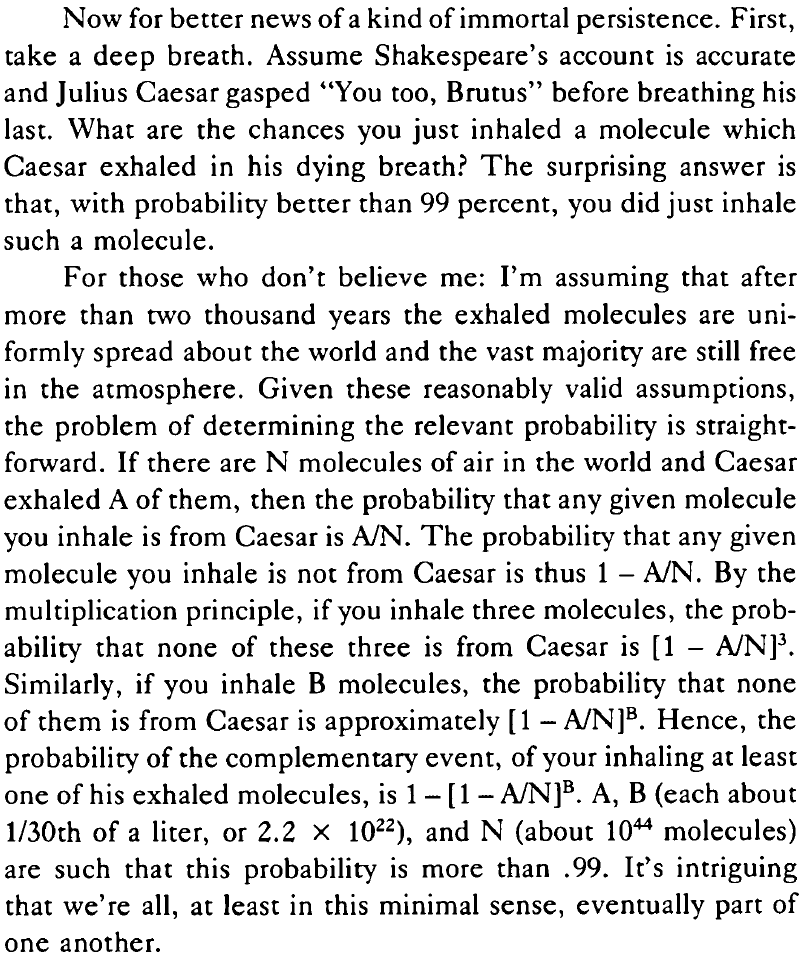
\includegraphics[width=0.8\linewidth]{images/caesar} \end{center}
\end{itemize}

\hypertarget{section-8}{%
\subsubsection*{61}\label{section-8}}
\addcontentsline{toc}{subsubsection}{61}

\begin{rmdbox}

\begin{itemize}
\item
  $n$ passageiros para $n$ assentos.
\item
  Passageiro $k$ inicialmente alocado no assento $k$.
\item
  MAS Passageiro $1$ decide escolher assento ao acaso (cada assento com a mesma probabilidade).
\item
  Então, cada passageiro seguinte se senta no assento inicialmente alocado para ele, se disponível; caso contrário, escolhe um assento ao acaso.
\item
  Qual a probabilidade de que o último passageiro se sente no assento alocado para ele?
\end{itemize}

\end{rmdbox}

\hypertarget{possibilidades}{%
\paragraph*{Possibilidades}\label{possibilidades}}
\addcontentsline{toc}{paragraph}{Possibilidades}

O último passageiro só pode se sentar no lugar $1$ ou no lugar $n$.

Aliás, isto é um caso específico de um fenômeno mais geral, Qualquer que seja o valor de $n$:

\begin{itemize}
\item
  O passageiro $3$ nunca fica no assento $2$: ou o passageiro $1$ pegou, ou ficou livre para o passageiro $2$ (que é obrigado a pegá-lo).
\item
  O passageiro $4$ nunca fica nos assentos $2$ nem $3$: ou o passageiro $1$ pegou o assento $3$, ou aconteceu um dos casos acima e o assento $3$ ficou livre para o passageiro $3$ (que é obrigado a pegá-lo).
\item
  O passageiro $5$ nunca fica nos assentos $2$ nem $3$ nem $4$: ou o passageiro $1$ pegou o assento $4$, ou aconteceu um dos casos acima e o assento $4$ ficou livre para o passageiro $4$ (que é obrigado a pegá-lo).
\item
  etc.
\item
  Seguindo o raciocínio, chegamos à conclusão de que o passageiro $n$ só pode ocupar o assento $1$ ou o assento $n$.
\end{itemize}

\hypertarget{probabilidades}{%
\paragraph*{Probabilidades}\label{probabilidades}}
\addcontentsline{toc}{paragraph}{Probabilidades}

\begin{itemize}
\item
  Examinando exemplos com $n \in \{3, 4, 5\}$, a probabilidade parece ser $1/2$.
\item
  Por quê?
\item
  O assento do passageiro $n$ depende da pergunta (no momento em que o passageiro $n$ vai se sentar)

  {\hl{``O assento $1$ já foi tomado?''}}

  cuja resposta é oposta à da pergunta

  {\hl{``O assento $n$ já foi tomado?''}}
\item
  Com que probabilidade a resposta a esta última pergunta é sim?
\item
  Em todos os passos anteriores, \protect\hyperlink{possibilidades}{como explicado acima em ``possibilidades''}, os assentos $1$ e $n$ sempre estão disponíveis para qualquer passageiro que vá escolher um assento ao acaso.
\item
  Como todos os assentos têm a mesma probabilidade de ser escolhidos, a probabilidade de o assento $1$ estar tomado é igual à probabilidade de o assento $n$ estar tomado.
\item
  Logo, a probabilidade de o passageiro $n$ acabar no assento $n$ é $1/2$.
\end{itemize}

\hypertarget{section-9}{%
\subsubsection*{62}\label{section-9}}
\addcontentsline{toc}{subsubsection}{62}

\hypertarget{probabilidade-condicional}{%
\chapter*{04: Probabilidade condicional}\label{probabilidade-condicional}}
\addcontentsline{toc}{chapter}{04: Probabilidade condicional}

\hypertarget{vuxeddeo-3}{%
\section*{Vídeo}\label{vuxeddeo-3}}
\addcontentsline{toc}{section}{Vídeo}

\begin{center} \url{https://youtu.be/P7NE4WF8j-Q} \end{center}

\hypertarget{exercuxedcios-3}{%
\section*{Exercícios}\label{exercuxedcios-3}}
\addcontentsline{toc}{section}{Exercícios}

\href{https://projects.iq.harvard.edu/files/stat110/files/strategic_practice_and_homework_2.pdf}{Enunciados (pdf).}

\hypertarget{homework-1}{%
\subsection*{Homework}\label{homework-1}}
\addcontentsline{toc}{subsection}{Homework}

\hypertarget{lewis-carroll}{%
\subsubsection*{3.1 Lewis Carroll}\label{lewis-carroll}}
\addcontentsline{toc}{subsubsection}{3.1 Lewis Carroll}

\begin{rmdbox}
A bag contains one marble which is either green or blue, with equal probabilities. A green marble is put in the bag (so there are $2$ marbles now), and then a random marble is taken out. The marble taken out is green. What is the probability that the remaining marble is also green?

This problem was first posed by Lewis Carroll in 1893.

\end{rmdbox}

\hypertarget{xadrez}{%
\subsubsection*{3.5 Xadrez}\label{xadrez}}
\addcontentsline{toc}{subsubsection}{3.5 Xadrez}

\begin{rmdbox}

You are going to play $2$ games of chess with an opponent whom you have never played against before (for the sake of this problem). Your opponent is equally likely to be a beginner, intermediate, or a master. Depending on which, your chances of winning an individual game are $90\%$, $50\%$, or $30\%$, respectively.

\begin{enumerate}
\def\labelenumi{\alph{enumi}.}
\item
  What is your probability of winning the first game?
\item
  Congratulations: you won the first game! Given this information, what is the probability that you will also win the second game (assume that, given the skill level of your opponent, the outcomes of the games are independent)?
\item
  Explain the distinction between assuming that the outcomes of the games are independent and assuming that they are conditionally independent given the opponent's skill level. Which of these assumptions seems more reasonable, and why?
\end{enumerate}

\end{rmdbox}

\hypertarget{exercuxedcios-do-livro-cap.-2}{%
\subsection*{Exercícios do livro (cap. 2)}\label{exercuxedcios-do-livro-cap.-2}}
\addcontentsline{toc}{subsection}{Exercícios do livro (cap. 2)}

\hypertarget{section-10}{%
\subsubsection*{2}\label{section-10}}
\addcontentsline{toc}{subsubsection}{2}

\hypertarget{section-11}{%
\subsubsection*{4}\label{section-11}}
\addcontentsline{toc}{subsubsection}{4}

\hypertarget{section-12}{%
\subsubsection*{9}\label{section-12}}
\addcontentsline{toc}{subsubsection}{9}

\hypertarget{section-13}{%
\subsubsection*{12}\label{section-13}}
\addcontentsline{toc}{subsubsection}{12}

\hypertarget{section-14}{%
\subsubsection*{14}\label{section-14}}
\addcontentsline{toc}{subsubsection}{14}

\hypertarget{section-15}{%
\subsubsection*{15}\label{section-15}}
\addcontentsline{toc}{subsubsection}{15}

\hypertarget{section-16}{%
\subsubsection*{16}\label{section-16}}
\addcontentsline{toc}{subsubsection}{16}

\hypertarget{section-17}{%
\subsubsection*{17}\label{section-17}}
\addcontentsline{toc}{subsubsection}{17}

\hypertarget{section-18}{%
\subsubsection*{29}\label{section-18}}
\addcontentsline{toc}{subsubsection}{29}

\hypertarget{referuxeancias}{%
\chapter*{Referências}\label{referuxeancias}}
\addcontentsline{toc}{chapter}{Referências}

\hypertarget{refs}{}
\begin{CSLReferences}{0}{1}
\leavevmode\vadjust pre{\hypertarget{ref-devlin-2010-pascal-fermat}{}}%
DEVLIN, K. \href{https://doi.org/10.5951/mt.103.8.0579}{The {P}ascal-{F}ermat Correspondence: How Mathematics Is Really Done}. \textbf{The Mathematics Teacher}, v. 103, n. 8, p. 579--582, abr. 2010.

\leavevmode\vadjust pre{\hypertarget{ref-oliveira-2004-analis}{}}%
OLIVEIRA MORGADO, A. C. DE et al. \textbf{An{á}lise combinat{ó}ria e probabilidade}. Rio de Janeiro: Impa / Vitae, 2004.

\leavevmode\vadjust pre{\hypertarget{ref-paulos-1988-innum}{}}%
PAULOS, J. A. \textbf{\href{http://gen.lib.rus.ec/book/index.php?md5=20A842C0E7EB7F8992EDDA0082E9B76F}{Innumeracy: Mathematical Illiteracy and Its Consequences}}. 1. ed. New York: Hill; Wang, 1988.

\end{CSLReferences}

\end{document}
